\documentclass[11pt]{article}
\usepackage{mathtools}
\usepackage{mdframed}
\usepackage{fullpage}
\usepackage{amsfonts}
\usepackage{tikz}
\usepackage{fancyhdr}
\usepackage{lastpage}


%edit this for each class
\newcommand\name{John Collin Vincent}
\newcommand\classname{Com S 311}
\newcommand\assignment{Homework 4}


\newcounter{excounter}
\setcounter{excounter}{1}
\newcommand\ques[2]{\vskip 1em  \noindent\textbf{\arabic{excounter}\addtocounter{excounter}{1}.} \emph{#1} \noindent#2}
\newenvironment{question}{\ques{}\begin{quote}}{\end{quote}}


\pagestyle{fancy}
\rfoot{\name, page \thepage/\pageref{LastPage}}
\cfoot{}
\rhead{}
\lhead{}
\renewcommand{\headrulewidth}{0pt}
\renewcommand{\footrulewidth}{0pt}
\DeclarePairedDelimiter\ceil{\lceil}{\rceil}
\DeclarePairedDelimiter\floor{\lfloor}{\rfloor}


\begin{document}


  {\bf \classname \hspace{1cm} \assignment\hfill \name}
  \vskip 2em


  \begin{question}
    \center
    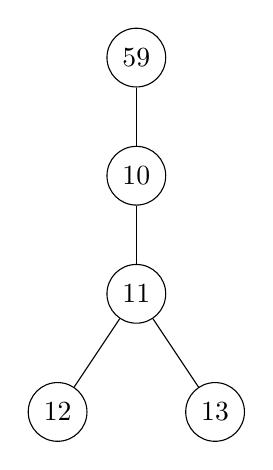
\begin{tikzpicture}[level/.style={sibling distance=60mm/#1}]
      \node [circle,draw] (z){$59$}
        child {node [circle,draw] (a) {$10$}
          child {node [circle,draw] (b) {$11$}
            child {node [circle,draw] (d) {$12$}}
            child {node [circle,draw] (e) {$13$}}
          }
        };
    \end{tikzpicture}
  \end{question}


\end{document}
